\documentclass[10pt]{article}
\usepackage{listings}
\usepackage{graphicx}
\usepackage{url}

% global commands

\newcommand{\javalst}[2]{
  \lstset{language=Java,captionpos=b,tabsize=4,frame=single,numbers=left,
    numberstyle=\tiny,numbersep=10pt,breaklines=true,showstringspaces=false,
    basicstyle=\footnotesize,emph={label}, caption={#1}, label={#2}}
}
\newcommand{\initlisting}[2]{
  \lstset{language={#1},captionpos=b,tabsize=4,frame=single,numbers=left,
    numberstyle=\tiny,numbersep=10pt,breaklines=true,showstringspaces=false,
    basicstyle=\footnotesize,emph={label}, caption={#2}}
}

\newcommand{\nm}{{\bf proTrade}}
\newcommand{\nmsp}{{\nm \ }}
% end commands
\setlength{\parskip}{0.3cm}
\setlength{\parindent}{0cm}

\begin{document}

\title{Report Three: Software Validation}

\author{Corina Ciobanu \and Iskander Orazbekov \and Mir Sahin \and Paul Grigoras \and Radu Baltean-Lugojan}

\date{\today}         % inserts today's date

\maketitle            % generates the title from the data above

\begin{abstract}
  \nmsp is a tennis trading environment which delivers the information a trader requires to place bets. Betting functionality, linked to the user's bank account is also provided. Testing and validation are crucial in order to deliver a reliable and secure application and have been used extensively.
\end{abstract}

\tableofcontents

\section{Introduction}
Tennis trading is a steadily growing market on the Betfair Exchange, with more than 70\% of bets being placed in-play. In order to maintain market liquidity, exchanges must attract customers for example, by supplying them with better tools. By providing more information and better visualization techniques such a tool can help the trader improve his understanding and predict the market evolution, which should (potentially) lead to an increased profit.

For tennis in particular, the information required to predict/understand the market evolution is the score, player statistics, potentially a live video feed of the match and, of course, the market data (evolution of betting odds). Ideally, this is desired for both historical and live matches.

At the moment, no application provides all this information. A number of solutions exist which allow visualization of historical market data, but they generally lack the more specific, tennis related data. For example in Fracsoft () market data is not correlated with match data (scores, player statistics). BetAngel() provides some tennis related data and prediction, but relies on the user to input the score, by pushing buttons, which is not suited for the speed at which the market can move. Ideally all the information should be automatically provided.

\nmsp means to fill this gap, by providing all the information, betting and prediction functionalities for both historical and live matches, in an entirely automated fashion.

Due to the ambitious nature of the project and the high risk associated with some user actions (e.g. placing bets with real money) in order to ensure reliability and stability testing and other validation methods have been used exstensively. 

\section{Testing}
Testing has been used throughout all stages of the project starting with iteration 4 and more extensively with the introduction of the Continuous Integration server in iteration 5.

As suggested in \cite{bk-testing} we have used the tests to guide our design, based on the principle that if a project is well designed it should be easy to write meaningful tests for it.

\textbf{Unit testing} has been used to rapidly test small portions of code while \textbf{acceptance tests} have been used to test a system feature from front to back. \textbf {TDD tests} (tests written before features) are expected to fail when they are written and should pass once the feature has been completely implemented. Once it passes, a test is transferred to the regression suite. Naturally, a failing \textbf{regression test} indicates a break in previous functionality (regression).

%\subsection{Preliminaries - Project Structure}

\subsection{Unit Testing}
Because of the ease of use, unit testing has been adopted early on in the development process and it has been of great use in identifying bugs and ensuring correctness of the Match API (an important set of classes which manages data such as score and statistics). 

Since tennis scoring rules are peculiar (for example points are counted 15, 30, 40, AD instead of just 1,2,3,4) and tests are particularly easy to write we adopted a TDD aproach. For example a simple initial test was written to verify the outcome of adding four consecutive points to one of the players: the player in cause should win the game which his game score, and resets the points score. Furthermore the oponnent's score should always be zero. The code for this is presented in \ref{list1}.

\javalst{Initial failing test for score. The initialisation of the score object is handled in an abstract super class which also provides assertSetScoreIs() and assertGamesScoreIs().}{list1}
\begin{lstlisting}
  @Test
  public void fortyZeroWin(){
    int expectedPoints[] = {15,30,40};
    for (int i=0;i<3;i++){
      score.addPlayerTwoPoint();
      assertGameScoreIs(0,0);
      assertPointsScoreIs(0, expectedPoints[i]);
    }
    score.addPlayerTwoPoint();
    assertGameScoreIs(0,1);
    assertPointsScoreIs(0,0);
  }
\end{lstlisting}

Having first written the test and ensured it failed, we then proceeded to designing and implementing a solution that would make it pass. 
We adopted this approach for the whole Match API and for the Prediction API (used to predict the evolution of a match based on current score and player statistics).

This approach helped us identify numerous bugs early on and guided us towards a better overal design of the APIs.

**e.g. a function for correctly setting a set score to a certain value was not initially provided, but since while writing the tests the need for such a function became obvious, it was included and tested**
** separate tests that measure progress from tests that catch regression **

\subsection{Acceptance Testing}
Acceptance tests were designed separately and were meant to test a particular function of the system, starting from the front-end (e.g. finding a pushing a button on the UI) to the back-end (e.g. connecting to the Betfair API to authorize a login request).

For performance reasons these were ran separately from unit tests since the UI operations tend to be slow.

For example the test in \ref{list2} checks the login functionality: the user should fill in their Betfair account and password and click on the login button. The login attempt is checked against the Betfair API and a label is updated to indicate success or failure. Obviously, an attempt to login with the test account should result in a success message being displayed.

\javalst{Initial failing test for the login window. The username and password for the test account are read and decrypted from a local config file by the Main class. Using the UI bot we then fill the data in on the login window and click the login button.}{list2}
\begin{lstlisting}
    @Test
    public void correctLoginSuccess() throws Exception {
        SWTBotText username = bot.text("username");
        username.setText(Main.getTestUsername());
        SWTBotText password = bot.text("password");
        password.setText(Main.getTestPassword());
        loginButton.click();
        SWTBotLabel success = bot.label(LoginShell.SUCCESS);
        assertNotNull(success);
    }
\end{lstlisting}

We have adopted a similar approach for all features.

However, due to limitations in the SWTBot API some features have proven impossible to test. For example we have not found a way to test the functions of a context menu (pop up) or a progress bar.

** new acceptance tests will not pass until the feature is implemented

acceptance tests for completed features catch regressions and should always pass (might take
longer to run)

once an acceptance test has passed, if it fails again that means a regression (the existing code has been broken)

SWTBot **

\subsection{Regression Testing}
As explained above(?), once a test has passed for the first time, it is moved to the regression suite.

Keeping failing tests (for features which have not been implemented) separate from passing tests is key in quickly identifying when a regression has occured.

Consequently we provide a task that automatically moves a test from the TDD suite to the regression suite.

The normal flow is: 
\begin{enumerate}
\item write a failing test (ensure it fails)
\item make the test pass
\item check for regression;
\item fix any regression
\item move test from TDD suite to regression suite
\item commit changes
\item repeat
\end{enumerate}

\subsection{Integration Testing}

Given the dependency on a large number of external APIs, we have used integration testing to ensure that these behave as expected and quickly identify potential configurarion issues. 

This has been done by writing tests that ensure the abstractions built on top of the libraries work as expected. To reduce coupling (and simplify the testing process), normally one interface and an implementation class expose the required functionality, encapsulating all other logic required for manipulating the library. As examples we discuss the testing approach for three of the most heavily used libraries: the Betfair API, SWT and SWTChart.

\subsubsection{Betfair API}

The Betfair API is organised in three services: global, UK Exchange and AUS Exchange, each defined through a WSDL(Web Service Description Language) specification. Our application only uses the first 2 services, accessed through Axis-generated Java classes, archived in generated.jar library.

Any connection to Betfair and use of the API is handled by classes in the src.model.connection package. Moreover, to ensure both services (Global and UK Exchange) only have one point of access, all the required functionality has been encapsulated in two classes - BetfairExchangeHandler and BetfairConnectionHandler. Hence, integration tests for these classes ensure the connection to the Betfair API works properly.

\subsubsection{SWT (?)}

How does SWT work?...

Since our project is not very large, we have considred acceptance tests are good/strong enough to test integration with the SWT platform/library.

\subsubsection{SWTChart}

How does SWTChart work?..

To ease our use of the SWTChart library and the ability/.. to add specific features required by our application, we have extended the Chart class of the SWTChart library. Hence, integration tests for this class ensure the library integrates smoothly into the entire application. 


\subsection{Continuous Integration}

Since the beginning of iteration 5 a continuous integration has been installed on a virtual machine provided by the Computing Support Group, which emulats a dual core, 1GB, 64bit machine.
We have decided to use Hudson, which comes with a plugin for running UI tests. These are different than normal tests since they require a display and cannot run on a headless server, unless some in memory display mechanism is provided. There are two alternatives: xvfb and hudson's plugin. Since we initially assumed xvfb would be harder to setup
Hudson provides easy integration with git.
The CI server is set to poll the repository and, when changes are detected, checks out a fresh copy and runs our normal build script.

\begin{figure}[ht]
\centering
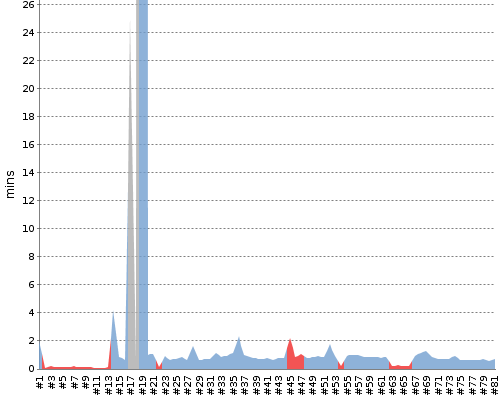
\includegraphics[bb=0 0 500 400, scale = 0.6]{build-trend.png}
\caption{Build trend summary. Vast majority of builds are well under 10 minutes. Outlying values were caused by a network outage.}
\end{figure}

\subsection{Measuring Test Coverage}

Since we did not adopt a TDD approach from the very beginning, it was important to obtain an overview of the parts of the code that need to be tested. Starting with iteration 5 we have used Cobertura,  an open source tool which provides neat test coverage reports for Java programs.

To facilitate report generation, a single ant task has been set up to compile the code with the debug info (vital for Cobertura to indicate line numbers and measure coverage), run all the tests (unit, acceptance, integration) and generate human readable reports which provide an indication of the current test coverage as well as branch coverage and complexity measures.

This data enabled us to identify lines which were not touched by tests. This is usually fixed by writting another test to cover the specific path, but it can also be the case that the functionality is actually never required, in which case it is completely removed. Again this illustrates how tests have been used to ensure a neat design/code etc. 

Branch coverage indicates when tests do not cover particular cases and has proven useful with regards to particularly tricky conditionals.

Cobertura also generates cyclomatic complexity values for each class/package, measuring the number of independent paths through the control flow graph of the code. Since it has been shown that high values are usually an indication of error prone code[2] this measurement is used to check code sanity.

\begin{figure}[ht]
\centering
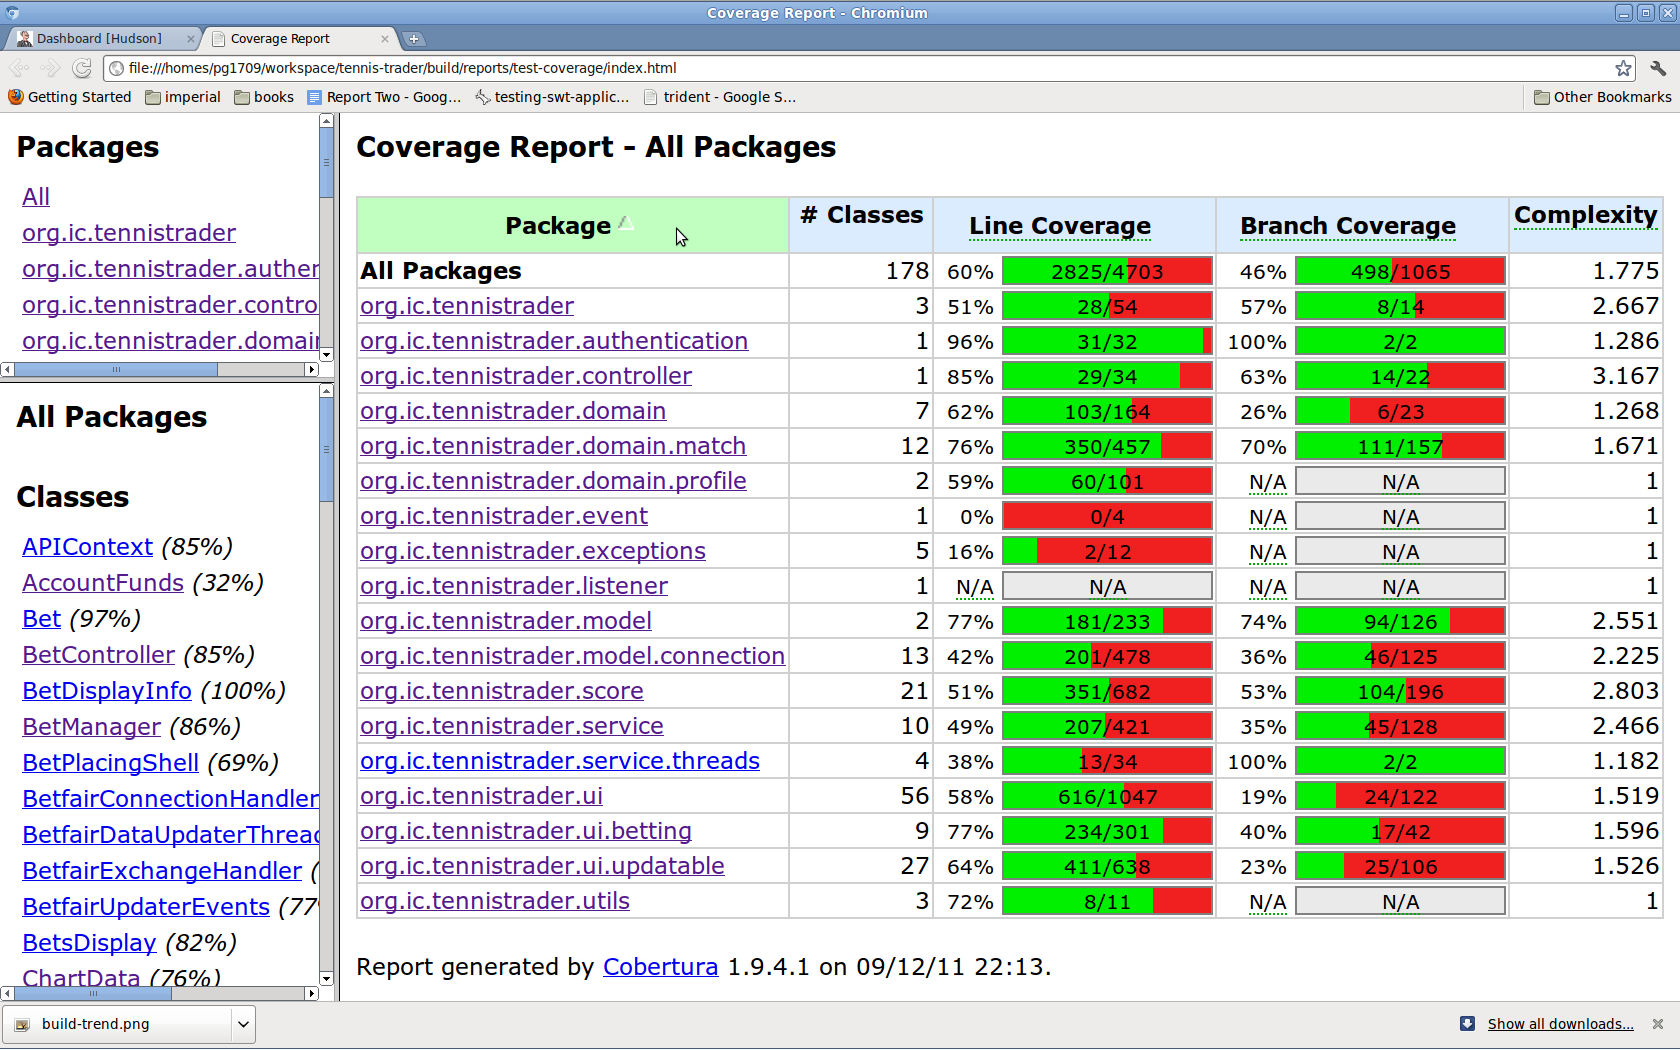
\includegraphics[bb=0 0 1680 1050, scale = 0.2]{coverage.png}
\caption{Coverage report generated by Cobertura indicates test coverage at package level, branch coverage an cyclomtic complexity.}
\end{figure}



\begin{figure}[ht]
\centering
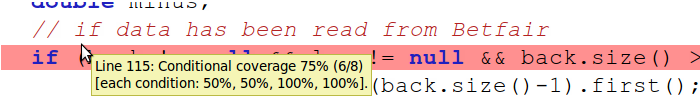
\includegraphics[bb=0 0 700 100, scale = 0.49]{branch.png}
\caption{Branch coverage indicates specific condition coverage.}
\end{figure}

\subsection{Code Sanity Measures}

We have used PMD to generate code sanity reports.

\begin{figure}[ht]
\centering
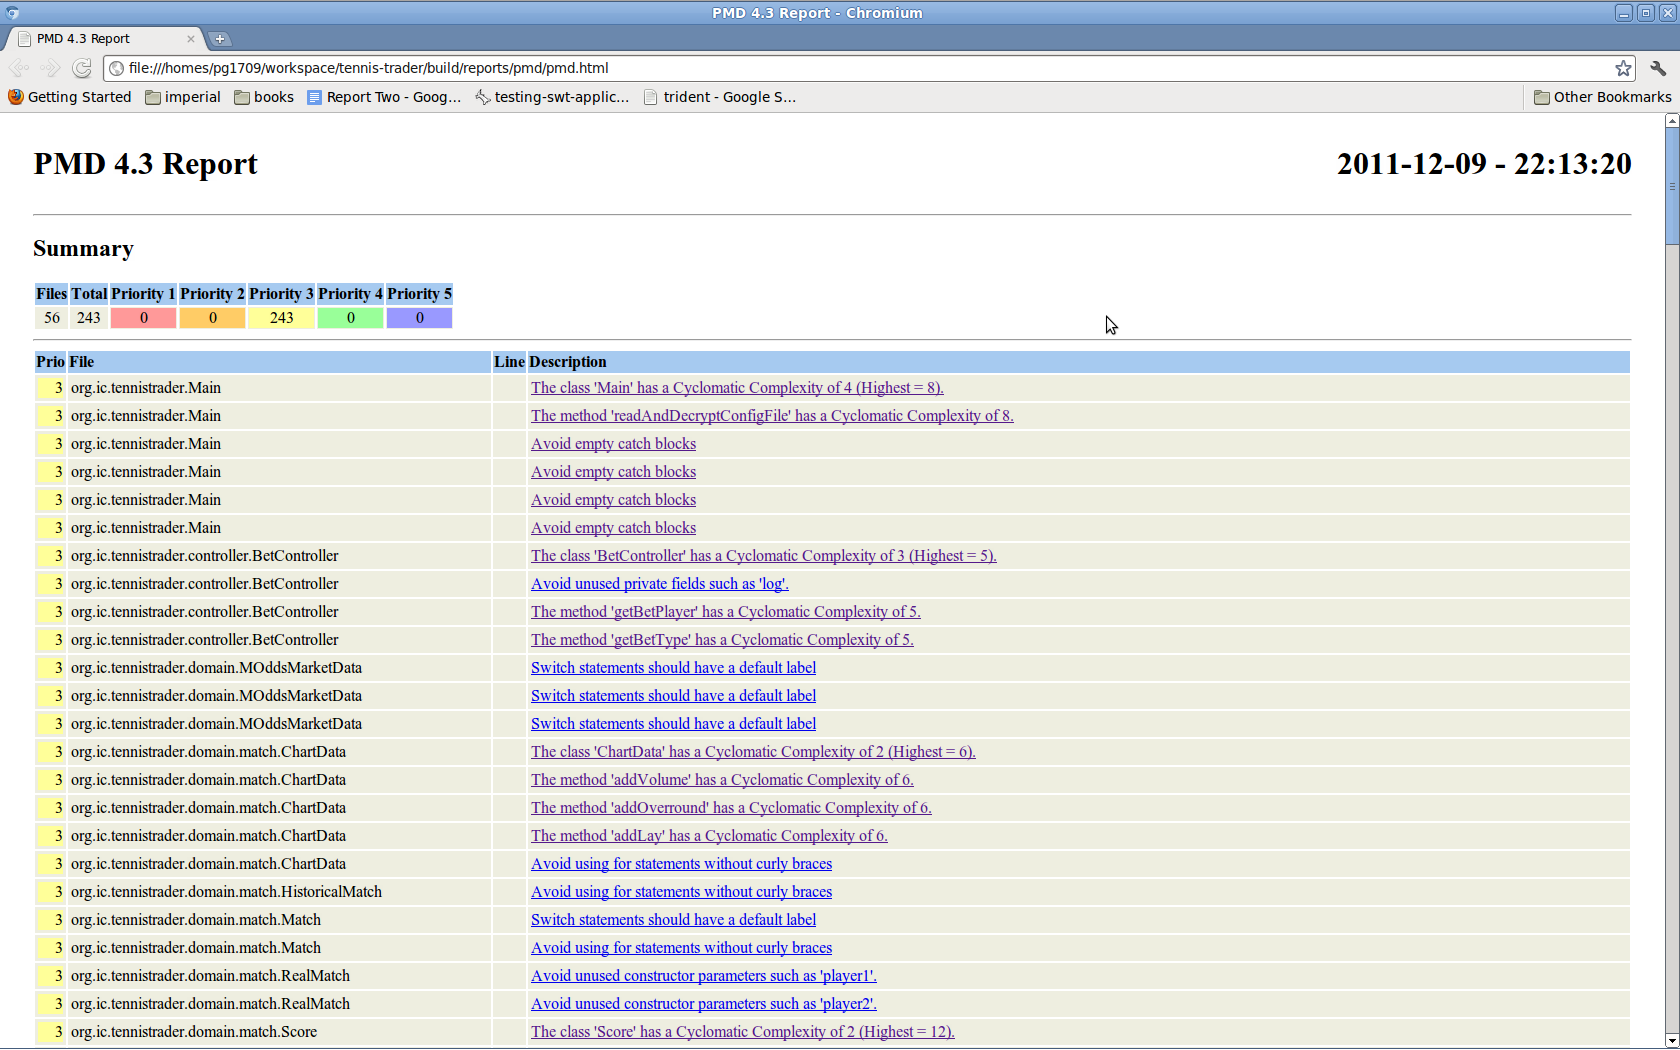
\includegraphics[bb=0 0 1680 1050, scale = 0.2]{pmd.png}
\caption{Branch coverage indicates specific condition coverage.}
\end{figure}

\subsection{Logging}

\subsection{Test Guided Design}
Refactoring

Used extract superclass, pull up (for tests), extract class

\subsection{At which development stages did you use tests? }

We have started using unit and regression tests as soon as the first cohesive draft of the Match API, containing all core features, was created (iteration 4). This allowed us to validate our design and do any major refactoring work around that stage. In the next iteration (5), testing has been supplemented with continuous integration and measuring code coverage to create test case improvements for more extensive coverage and system integration on our current version and throughout our future iterations. After obtaining all necessary data for buiding the Prediction API, further unit and regression tests have been developed as it was being developed, leading to a TDD approach for the latter part of the project.

\subsection{Portions of code base tested}

All core components of the proTrade application have clear distinctions between back/front ends, local/enternal data, and internal state/state handler-updater. The modular design is in direct relation with testing methodologies chosen, with unit tests validating the former ends and functional/acceptance tests testing the latter. On top, integration tests are used to reproduce and analyse behaviour of specific GUI or data fetching/updating libraries that are used in conjunction with local features. A functional overview of the applications's code base and features together with their tests is given below:

\begin{itemize}
\renewcommand{\labelitemi}{$\bullet$}
\item Authentication: Encrypt/decrypt functions for storing and accessing the login credentials are unit tested, while the interface (LoginShell) is acceptance tested (as detailed in section 2.2).
\item Controller: The bet controller, built upon relevant back/lay buttons and their associated functionality of placing bets, is tested functionaly in 'BetControllerTest' for correct bet types and player recognition
\item Domain/Match: Local functionality of populating/retrieving the chart widget with market data is unit tested in 'ChartDataTest'
\item Model: The internal state representation relating to player data and matched/unmatched bets corresponding to the market/user are unit tested, while the exchange connection that updates the internal state is validated via functional tests.     
\item Score: Front end 'PredictionGui' controller is functionally tested, whereas specific unit tests are written for back-end components such as statistics fetching and parsing or the 'PredictionCalculator' model. 
\item Service: Since this package models the back end receiver for various incoming data, state updating is unit tested and integration with BetFair API services is checked
\item UI: Acceptance and integration testing of all front-end GUI interfaces
\item UI-Betting/Updatable: Integration testing on dynamical GUI elements driven by user input or data updates
\end{itemize}

\begin{figure}[ht]
\begin{center}$
\begin{array}{ccc}
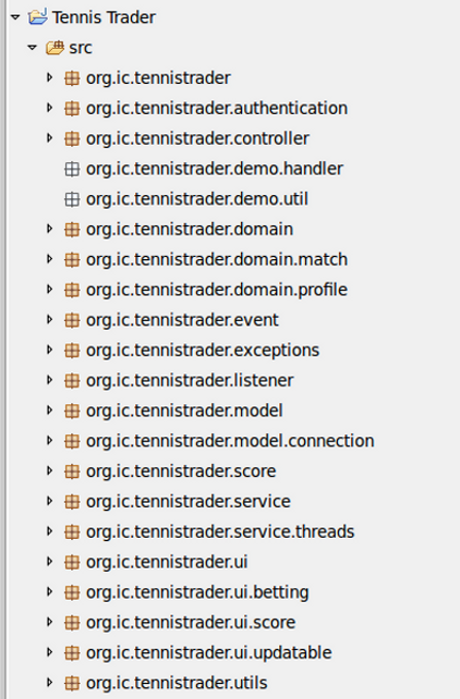
\includegraphics[bb=0 0 499 700, scale = 0.25]{project.png} &
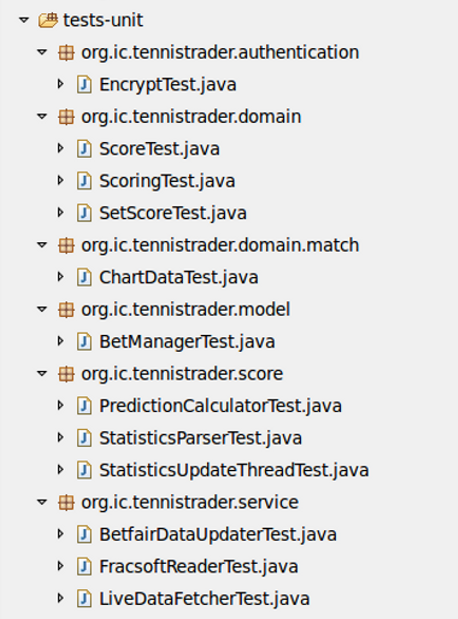
\includegraphics[bb=0 0 499 700, scale = 0.25]{tests-unit.png} &
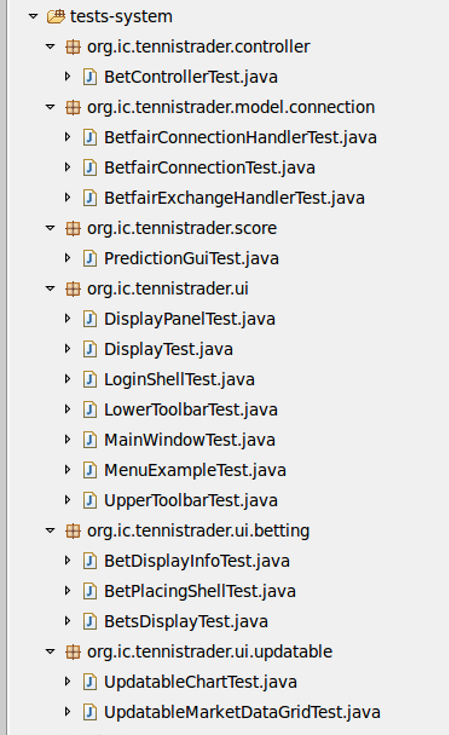
\includegraphics[bb=0 0 499 700, scale = 0.25]{tests-system.png} 
\end{array}$
\end{center}
\caption{Left - Project hierarchy with included packages. Center - Unit tests for local functionality/model based classes/packages. Right - System tests for controller/UI oriented classes/packages}
\end{figure}

\subsection{Bugs/problems revealed by testing}

Apart from validating design, testing has revealed hidden bugs in various components of the system. 

Unit tests have invalidated a first encoding of the scoring system for the prediction calculator, when translating between traditional tennis point scores and an incremental representation. Furthermore, they have revealed some overlooked considerations in recursive state passing when computing a set prediction based on a Markov chain model, which led to wrong set winning probability estimates. 

\section{General Validation}
General Validation: to decribe any other methods you may have used to validate your executable deliverable; the following list is only suggestive but should give you an idea of what things you could do:

\subsection{User interface design validation}

The user interface of our application has been designed with a view towards obtaining a final product which achieves the following goals: it is visually eye-pleasing, it is simple to use, it minimizes the effort it takes for users to accomplish their work/wish/..
To the purpose of validating our user interface design, feedback has been collected from a number of different persons with or without experience in using trading applications.

\subsubsection{Feedback experienced users}

Firstly, we have had constant feedback from our supervisor, who is familair with the game of tennis and tennis betting and who understands the needs of a professional trader. He has guided us through the process and has pointed out a number of possible UI improvements along the way (such as positioning different components, displaying different data on the graph), which we have accomplished.

Secondly, we have had meetings with PhD students, who are themselves developing trading applications. They gave us valuable feedback regarding market information display and the best way to present it to a specialized user. Hence, our initial interface has been adapted to accommodate their suggestions (e.g. displaying some additional market statistics) - supported by our supervisor.

Finally, to collect feedback from other points of view as well, our supervisor arranged for us to meet the head of research of Betfair. He has approved(?) of our application's general interface and pointed out a few possible issues (such as synchronizing all the playback data), which are now fixed(?).

\subsubsection{Feedback unexperienced users}

To test how easy it is for users to understand the information presented by our application and how ''natural'' to find the required functionalities, we have collected feedback from a few colleagues, without previous experience with tennis trading applications. (??? - what did they say?)

Overall, the interface of our application has been validated by the users, with some improvement suggestions which we have considered and implemented.


\subsection{Did you use lint or similar tools?}

We used PMD and Cobertura report to check code ``sanity''.

\subsection{Did you conduct a manual code inspection (not by the person who wrote the code)?}

We also used a review mechanism in which, normally, code has been inspected by at least two team members.

\subsection{Did you exert your software to stress testing?}

No - should do.

\subsection{Did you test the GUIs of your software?}
Yes, as explained above we have test the UI through our acceptance tests. Also visual inspection by team members was used to ensure no layouts are messed up.

yeees

\section{Managerial Documentation}

This section provides a formal account of group management and activities.

\subsection{Collaboration Tools}

Throughout the project various collaboration tools were used that would help in cooperation for successful product delivery.

Use of git significantly improved the quality of work produced by the team, as it provided not only a shared code base with version control, but also a good picture of the current state of the project. Moreover, it encouraged team members to use “Commit Early, Commit Often” paradigm, as many postponed commits tended to result in a large number of merge conflicts. As a consequence of an increase in the commit frequency, the monitoring capability of the project also raised, simplifying error tracking and resolving.

Furthermore, a private github repository was created, providing the team with a set of features that supported further collaboration. First of all, team used issues that could be tracked and assigned to specific group members. These tasks had comment threads linked to them, simplifying communication and giving an ability to have almost instant feedback on the solution. Moreover, use of issues dramatically increased working efficiency of the team, for example, whenever there was a new issue added to the back log, all teammates were notified, and once one of them has finished work on his or her piece, this member could then start thinking on another problem. As well as that, github repository provided the ability to split issues into different milestones, consequently providing better sense of direction for everyone in the group. As a result, it helped to enforce the agile development paradigm, making it possible to have distinct iterations, thus increasing the level of cooperation between team members.

Another set of collaboration tools that proved to be useful was google docs. This platform allowed the whole group to exchange information by creating files accessible to the whole group. The team primarily used it to make meetings agendas, keep logs of the work done via tables and set global objectives for particular iterations. The use of google docs also simplified report editing because of the instant feedback and constant monitoring of the different sections by other team members.

In order to share more specific information and larger files, team members had dropbox accounts. This allowed to share data related to tennis, sports trading, Betfair API and particular software libraries, for example GUI libraries for chart display.

To establish a concrete communication channel throughout the project group, it was essential to have a good media that everyone would have an access to. First of all, emails provided good updates for the whole team and simplified the process of making proposals and raising issues that needed consideration of all team members. Skype and IM services, in turn, made it easier for several group members to work on specific issues and provided an excellent media for knowledge exchange.

\subsection{Management Policies}

Agile Project Management

\subsubsection{Code Change Policy}

\subsubsection{Validation Policy}

\subsection{Knowledge Transfer}


A table of the group meetings - including dates, format and which members attended
A table of the hours spent per week on which tasks or activities by each member on the project
The Log-Book


Evaluation Criteria for Report Three: the same as for Reports One and Two.

\begin{thebibliography}{9}
\bibitem{bk-testing}
  Steeve Freeman, Nat Pryce,
  \emph{Growing Object-Oriented Software, Guided by Tests}, Addison-Wesley 2010

\bibitem{web-cyccom}
  Robert Chatley's course on Software Engineering Methods
  \url{http://en.wikipedia.org/wiki/Cyclomatic_complexity},
  Imperial College London

\bibitem{bk-aglsam}
  Jonathan Rasmusson,
  \emph{The Agile Samurai},
  Pragmatic Bookshelf,
  October 2010.

\bibitem{bk-aglflh}
  Jeff Langr and Tim Ottinger,
  \emph{Agile in a Flash},
  Pragmatic Bookshelf, 
  January 2011.

\bibitem{web-rbc}
  Robert Chatley's course on Software Engineering Methods
  \url{http://www.doc.ic.ac.uk/~rbc/302/},
  Imperial College London

\end{thebibliography}

\end{document}
